%  Zostavený pre predmet Neurónové siete 2025/2026
\documentclass[12pt,a4paper]{article}

\usepackage[utf8]{inputenc}
\usepackage[T1]{fontenc}
\usepackage[main=slovak]{babel}
\usepackage{geometry}
\usepackage{booktabs}
\usepackage{graphicx}
\usepackage{amsmath}
\usepackage{amssymb}
\usepackage{hyperref}
\usepackage{float}
\usepackage{subcaption}
\usepackage{caption}
\usepackage{array}
\usepackage{multirow}
\usepackage{xcolor}
\usepackage{listings}
\usepackage{parskip}

\geometry{
  a4paper,
  top=2.5cm,
  bottom=2.5cm,
  left=3cm,
  right=2.5cm,
}

\hypersetup{
  colorlinks=true,
  linkcolor=blue,
  citecolor=blue,
  urlcolor=blue,
}

% -----------------------------------------------------------------------
\title{
  \textbf{Súboj generácií ResNet:} \\
  \large Vplyv hĺbky na stabilitu učenia
}
\author{Marko Zeliznak \and Daniel Szabo \and Samuel Labanc \and Samuel Stefan}
\date{Neurónové siete 2025/2026 \\ \today}
% -----------------------------------------------------------------------

\begin{document}

\maketitle
\tableofcontents
\newpage

% ======================================================================
\section{Formulácia problému}
% ======================================================================

Tento projekt sa zameriava na porovnanie dvoch reziduálnych konvolučných neurónových sietí
— \textbf{ResNet-34} a \textbf{ResNet-50} — pri klasifikácii obrazov na datasete CIFAR-10.
Centrálna výskumná otázka znie:

\begin{quote}
\textit{Ako zmena hĺbky siete (ResNet-34 vs. ResNet-50) ovplyvňuje stabilitu učenia,
rýchlosť konvergencie, pamäťovú náročnosť a dosiahnutú presnosť klasifikácie?}
\end{quote}

Kľúčová motivácia vychádza z paradoxu hlbokých sietí: intuitívne by sme očakávali,
že hlbšia sieť s väčším počtom vrstiev dosiahne lepšie výsledky. V praxi však samotné
pridávanie vrstiev spôsobuje problémy (miznúci/explodujúci gradient, degradácia presnosti).
Architektúra ResNet tento paradox adresuje reziduálnymi prepojeniami (\textit{skip connections}).
Zaujíma nás, či prechod od ResNet-34 k ResNet-50 prináša merateľný prínos, alebo či zvýšená
výpočtová náročnosť nie je oprávnená pri jednoduchšom datasete (CIFAR-10).

Sekundárnou výskumnou otázkou je \textbf{ablačná štúdia vplyvu rýchlosti učenia} (learning rate):
porovnávame hodnoty $lr = 10^{-3}$ a $lr = 10^{-4}$ pre obe architektúry, čím sledujeme
interakciu hĺbky siete s voľbou hyperparametru.

% ======================================================================
\section{Teoretické pozadie}
% ======================================================================

\subsection{Problém miznúceho gradientu}

Pri spätnom šírení chyby (\textit{backpropagation}) sa gradient znásobuje
Jacobiánom každej vrstvy. Ak sú tieto hodnoty menšie ako 1, gradient exponenciálne
klesá smerom k vstupným vrstvám — hovoríme o \textit{miznúcom gradiente} \cite{hochreiter1991}.
Výsledkom je, že skoré vrstvy sa učia extrémne pomaly, čím celkové trénovanie stagnuje.
Opačný jav, \textit{explodujúci gradient}, nastáva keď sú hodnoty Jacobiánov väčšie ako 1.

\subsection{Reziduálne prepojenia (Skip Connections)}

Architektúra ResNet \cite{he2016deep} rieši oba problémy zavedením reziduálneho bloku:
\begin{equation}
  \mathbf{y} = \mathcal{F}(\mathbf{x},\, \{W_i\}) + \mathbf{x}
\end{equation}
kde $\mathcal{F}(\mathbf{x})$ je reziduálna funkcia (niekoľko konvolučných vrstiev)
a $\mathbf{x}$ je vstup prenesený priamo cez skok (\textit{identity shortcut connection}).
Tento tvar má niekoľko dôsledkov:
\begin{itemize}
  \item Gradient môže plynúť priamo cez skratku bez útlmu.
  \item Sieť sa môže naučiť iba reziduálnu diferenciu oproti identite — jednoduchšia úloha.
  \item Hlbšie siete prestávajú degradovať: pridanie vrstiev nemôže zhoršiť výsledky,
        lebo v najhoršom prípade sa naučia nulový reziduál ($\mathcal{F} = 0$).
\end{itemize}

\subsection{ResNet-34 vs. ResNet-50}

\paragraph{ResNet-34} používa \textit{základné reziduálne bloky} (\textit{basic blocks})
tvorené dvoma konvolúciami $3 \times 3$ za sebou:
\begin{equation}
  \text{BasicBlock}: \quad \text{Conv}_{3\times3} \to \text{BN} \to \text{ReLU}
                        \to \text{Conv}_{3\times3} \to \text{BN} \to (+\,x) \to \text{ReLU}
\end{equation}

\paragraph{ResNet-50} nahradí základné bloky \textit{bottleneck blokmi}, ktoré
znižujú dimenziu príznakových máp pred drahšou $3 \times 3$ konvolúciou a potom
ju opäť rozširujú:
\begin{equation}
  \text{Bottleneck}: \quad \text{Conv}_{1\times1} \to \text{BN} \to \text{ReLU}
                        \to \text{Conv}_{3\times3} \to \text{BN} \to \text{ReLU}
                        \to \text{Conv}_{1\times1} \to \text{BN} \to (+\,x) \to \text{ReLU}
\end{equation}

Bottleneck bloky umožňujú väčšiu hĺbku bez dramatického nárastu FLOP-ov na blok,
avšak zvyšujú celkové parametre a pamäťovú náročnosť siete.

\subsection{Adaptácia pre CIFAR-10}

Originálny ResNet bol navrhnutý pre ImageNet (obrázky $224 \times 224$). Pri priamom
použití na CIFAR-10 ($32 \times 32$) by prvá konvolúcia $7 \times 7$, stride 2 s
následným max-poolingom (stride 2) zredukovala priestorové rozlíšenie na $8 \times 8$
ešte pred prvým reziduálnym blokom, čím by sa stratila podstatná časť informácie.
Preto sme predradenosť adaptovali:
\begin{itemize}
  \item \texttt{conv1}: $7 \times 7$, stride 2 $\to$ $3 \times 3$, stride 1 (zachováme rozlíšenie)
  \item \texttt{maxpool}: nahradená identitou (žiadne downsampling)
\end{itemize}
Táto adaptácia je štandardným prístupom pre CIFAR-10 \cite{he2016deep}.

\subsection{Optimalizátor a plánovač}

Použili sme \textbf{Adam} \cite{kingma2015adam} s reguláciou váh (\textit{weight decay} $10^{-4}$),
pretože Adam adaptívne škáluje rýchlosť učenia pre každý parameter.
Ako plánovač sme zvolili \textbf{CosineAnnealingLR} \cite{loshchilov2017sgdr}:
\begin{equation}
  \eta_t = \eta_{\min} + \frac{1}{2}(\eta_{\max} - \eta_{\min})
           \left(1 + \cos\!\left(\frac{t \cdot \pi}{T_{\max}}\right)\right)
\end{equation}
kde $T_{\max}$ je celkový počet epoch. Tento plán hladko znižuje rýchlosť učenia
a zabraňuje osciláciám na konci trénovania.

% ======================================================================
\section{Popis datasetu a predspracovanie dát}
% ======================================================================

\subsection{CIFAR-10}

CIFAR-10 \cite{krizhevsky2009learning} je štandardný benchmark pre klasifikáciu obrazov:
\begin{itemize}
  \item $60\,000$ farebných obrázkov ($32 \times 32$ pixelov, 3 kanály)
  \item 10 tried: \textit{airplane, automobile, bird, cat, deer, dog, frog, horse, ship, truck}
  \item $6\,000$ obrázkov na triedu (rovnomerné zastúpenie)
  \item Oficiálne rozdelenie: $50\,000$ trénovacích a $10\,000$ testovacích vzoriek
\end{itemize}

\subsection{Rozdelenie dát}

Aby sme zabránili úniku informácií (\textit{data leakage}), testovacia sada zostala
úplne oddelená počas celého trénovania. Validačnú sadu sme vyčlenili
z trénovacej množiny (10\,\% = $5\,000$ vzoriek), pričom rozdelenie bolo deterministické
(seed = 42) pre plnú reprodukovateľnosť.

\begin{table}[H]
\centering
\caption{Rozdelenie datasetu CIFAR-10}
\begin{tabular}{lrr}
\toprule
\textbf{Množina} & \textbf{Počet vzoriek} & \textbf{Účel} \\
\midrule
Trénovacia  & 45\,000 & tréning váh \\
Validačná   &  5\,000 & ladenie hyperparametrov, early stopping \\
Testovacia  & 10\,000 & finálna evaluácia (použitá iba raz) \\
\bottomrule
\end{tabular}
\end{table}

\subsection{Augmentácia a normalizácia}

Pri trénovaní sme aplikovali štandardnú augmentáciu:
\begin{itemize}
  \item \texttt{RandomCrop(32, padding=4)}: náhodné orezanie so zapadovaním
  \item \texttt{RandomHorizontalFlip()}: náhodné horizontálne zrkadlenie
\end{itemize}
Pri validácii a testovaní sme augmentáciu vypli.

Všetky obrázky sme normalizovali hodnotami odvodenými z trénovacej sady CIFAR-10:
\begin{equation}
  \mu = (0.4914,\; 0.4822,\; 0.4465), \qquad \sigma = (0.2470,\; 0.2435,\; 0.2616)
\end{equation}

% ======================================================================
\section{Metodológia}
% ======================================================================

\subsection{Implementačné rozhodnutia}

Modely boli implementované pomocou knižnice \texttt{torchvision.models} (PyTorch)
— bez trénovania od nuly z architektúry vlastnej implementácie, čo redukuje
implementačné chyby. Namiesto transfer learningu (ImageNet váhy) sme použili
\textbf{náhodne inicializované váhy} (Kaiming normal), pretože cieľom je porovnanie
architektúr, nie transfer learningu.

\subsection{Spoločné podmienky pre obe architektúry}

Aby bolo porovnanie spravodlivé, obe siete boli trénované za identických podmienok:

\begin{table}[H]
\centering
\caption{Konfigurácia trénovania (rovnaká pre oba modely)}
\begin{tabular}{ll}
\toprule
\textbf{Hyperparameter} & \textbf{Hodnota} \\
\midrule
Počet epoch       & 20 \\
Batch size        & 128 \\
Weight decay      & $10^{-4}$ \\
Optimalizátor     & Adam \\
Plánovač LR       & CosineAnnealingLR ($\eta_{\min} = 0$) \\
Seed              & 42 \\
Augmentácia       & RandomCrop + RandomHorizontalFlip \\
\bottomrule
\end{tabular}
\end{table}

\subsection{Sledované metriky}

Počas každej epochy sme zaznamenávali:
\begin{itemize}
  \item \textbf{Train/Val loss} (cross-entropy)
  \item \textbf{Train/Val accuracy} (\% správne klasifikovaných)
  \item \textbf{Gradient norm} (priemerná L2-norma gradientov cez všetky batchy)
  \item \textbf{Čas epochy} (sekundy)
  \item \textbf{Peak GPU pamäť} (MB)
\end{itemize}
Tieto metriky umožňujú nielen porovnanie finálnej presnosti, ale aj analýzu dynamiky
trénovania — dôležitého aspektu pri skúmaní vplyvu hĺbky na stabilitu.

% ======================================================================
\section{Návrh experimentov}
% ======================================================================

\subsection{Experimenty}

Realizovali sme 4 experimenty usporiadané v mriežke $2 \times 2$:

\begin{table}[H]
\centering
\caption{Prehľad experimentov}
\begin{tabular}{llll}
\toprule
\textbf{ID} & \textbf{Model} & \textbf{LR} & \textbf{Kód} \\
\midrule
E1 & ResNet-34 & $10^{-3}$ & \texttt{resnet34\_lr1e3} \\
E2 & ResNet-34 & $10^{-4}$ & \texttt{resnet34\_lr1e4} \\
E3 & ResNet-50 & $10^{-3}$ & \texttt{resnet50\_lr1e3} \\
E4 & ResNet-50 & $10^{-4}$ & \texttt{resnet50\_lr1e4} \\
\bottomrule
\end{tabular}
\end{table}

\subsection{Ablačná štúdia: vplyv rýchlosti učenia}

Porovnanie E1 vs. E2 (resp. E3 vs. E4) tvorí \textbf{kontrolovaný experiment}
(ablation study): meníme iba jeden hyperparameter (learning rate), zatiaľ čo
všetky ostatné podmienky zostávajú rovnaké. Cieľom je oddeliť vplyv architektúry
od vplyvu rýchlosti učenia.

Voľba hodnôt $10^{-3}$ a $10^{-4}$ je motivovaná tým, že pri Adame s CosineAnnealingLR
sú to reprezentatívne zástupcovia „rýchleho" a „pomalého" učenia na tejto škále.

% ======================================================================
\section{Výsledky}
% ======================================================================

\subsection{Porovnanie finálnych výsledkov}

\begin{table}[H]
\centering
\caption{Súhrnné výsledky všetkých experimentov}
\begin{tabular}{llccccc}
\toprule
\textbf{Experiment} & \textbf{Model} & \textbf{LR} &
\textbf{Best Val Acc} & \textbf{Test Acc} &
\textbf{Pamäť [MB]} & \textbf{Čas/ep. [s]} \\
\midrule
E1 & ResNet-34 & $10^{-3}$ & 92.54\,\% & \textbf{91.69\,\%} & 1\,338.6 & $\approx 45$ \\
E2 & ResNet-34 & $10^{-4}$ & 85.84\,\% & 85.19\,\% & 1\,336.6 & $\approx 45$ \\
E3 & ResNet-50 & $10^{-3}$ & 92.14\,\% & 90.96\,\% & 3\,526.5 & $\approx 72$ \\
E4 & ResNet-50 & $10^{-4}$ & 77.02\,\% & 77.25\,\% & 3\,525.7 & $\approx 72$ \\
\bottomrule
\end{tabular}
\end{table}

Najlepší výsledok dosiahol \textbf{ResNet-34 s lr = $10^{-3}$} (test acc 91.69\,\%).
ResNet-50 s rovnakou rýchlosťou učenia zaostal o 0.73 percentuálneho bodu.
Výraznejší rozdiel nastáva pri nižšom learning rate — ResNet-50 s $lr = 10^{-4}$
dosiahol iba 77.25\,\%, čo je o 7.94 p.b. menej ako ResNet-34 pri rovnakej LR.

\subsection{Krivky straty a presnosti}

\begin{figure}[H]
  \centering
  \begin{subfigure}[b]{0.48\textwidth}
    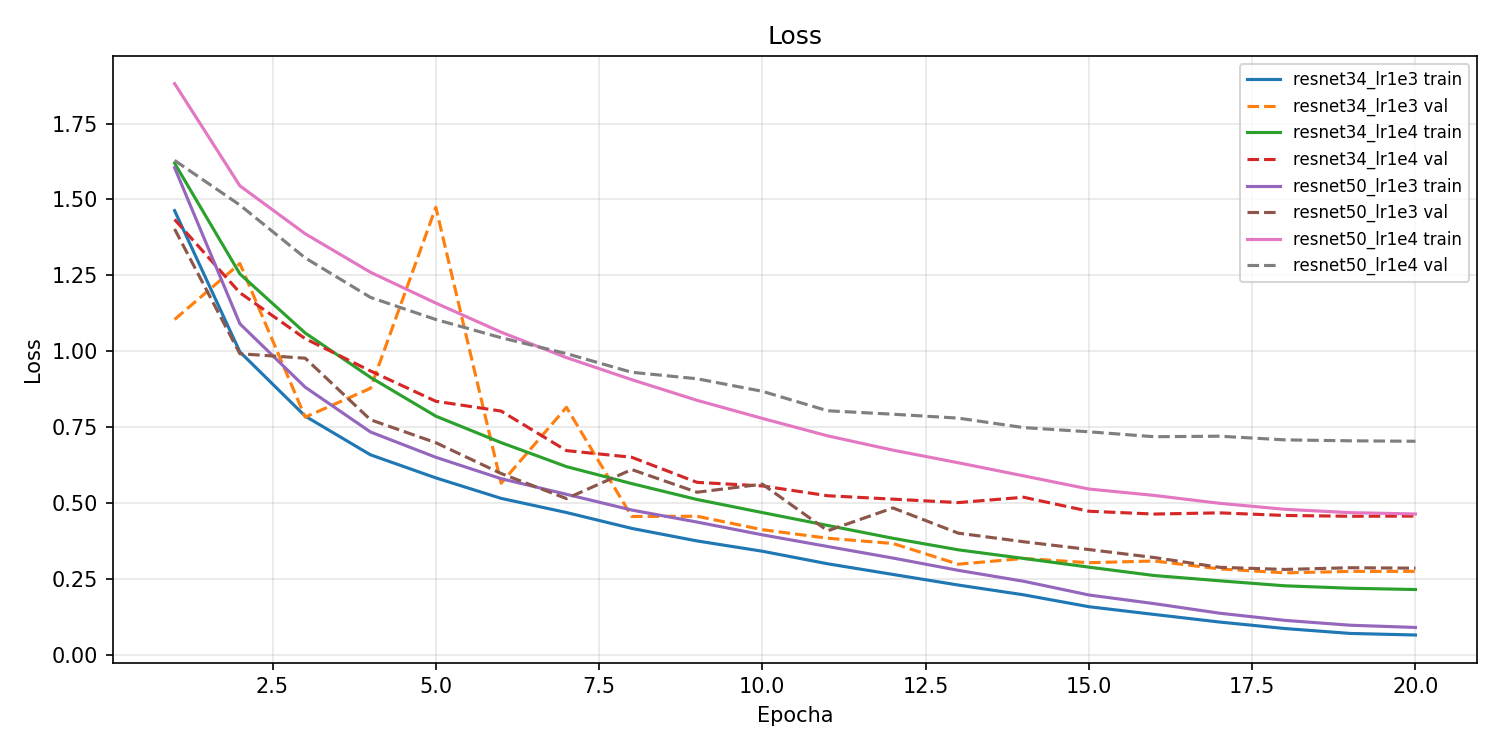
\includegraphics[width=\textwidth]{images/comparison_train_loss.png}
    \caption{Trénovacia strata (train loss)}
  \end{subfigure}
  \hfill
  \begin{subfigure}[b]{0.48\textwidth}
    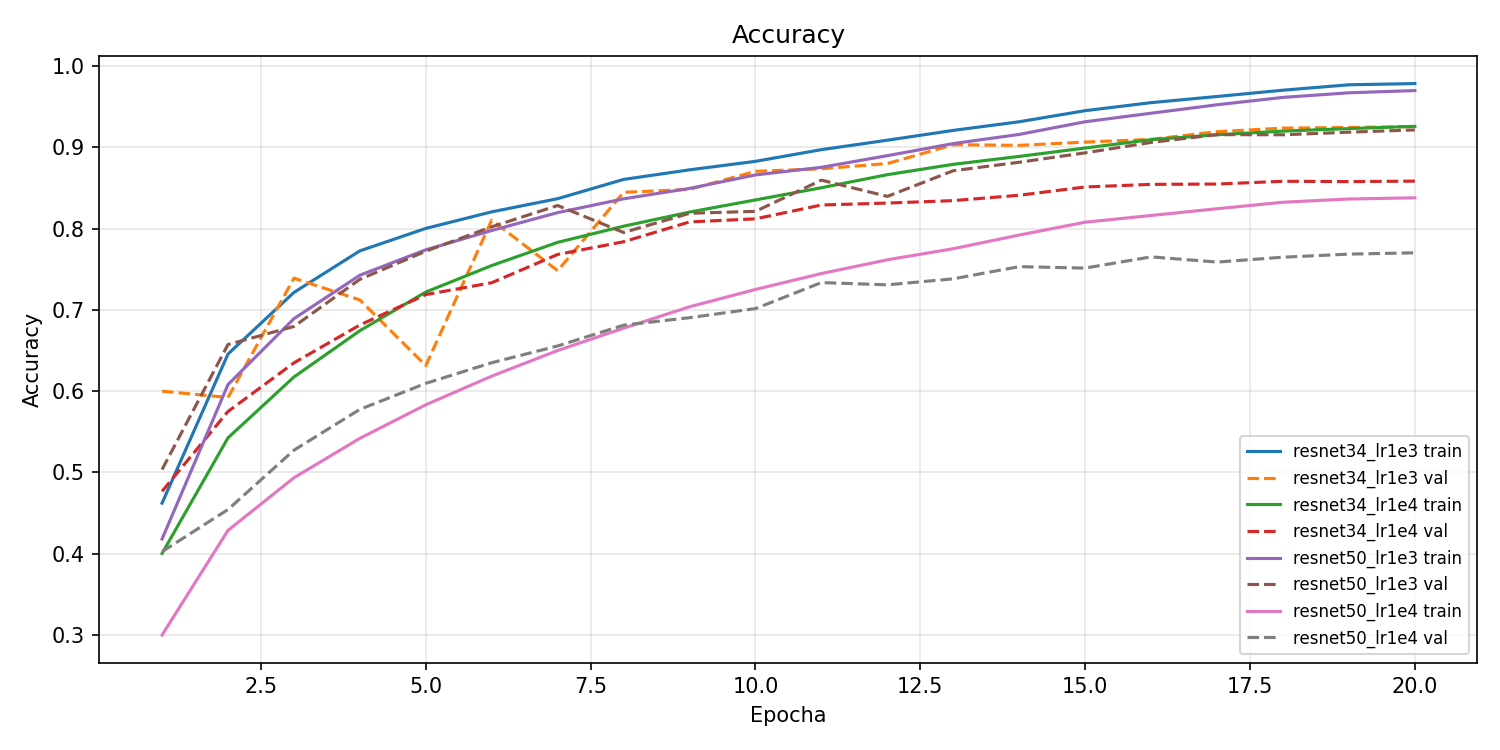
\includegraphics[width=\textwidth]{images/comparison_train_accuracy.png}
    \caption{Trénovacia presnosť (train accuracy)}
  \end{subfigure}
  \caption{Porovnanie priebehu trénovania pre všetky 4 experimenty (20 epoch)}
  \label{fig:loss_acc}
\end{figure}

Z obrázku \ref{fig:loss_acc} je zrejmé:
\begin{itemize}
  \item E1 a E3 ($lr = 10^{-3}$) konvergujú rýchlo a stabilne.
  \item E2 ($lr = 10^{-4}$, ResNet-34) konverguje pomaly ale monotónne.
  \item E4 ($lr = 10^{-4}$, ResNet-50) konverguje výrazne pomalšie — po 20 epochách
        ešte stále nedosiahol plochu konvergencie.
\end{itemize}

\subsection{Gradient norm}

\begin{figure}[H]
  \centering
  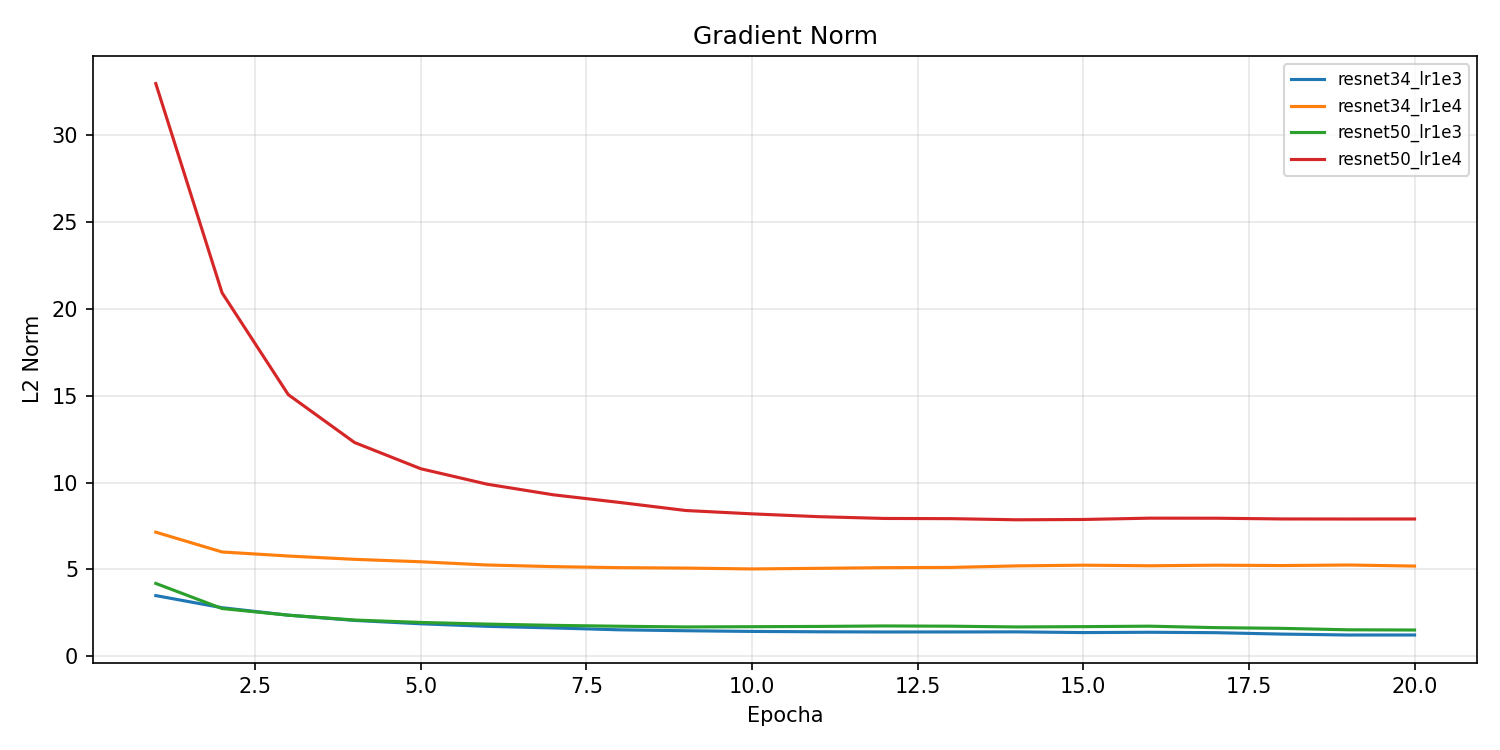
\includegraphics[width=0.65\textwidth]{images/comparison_gradient_norm.png}
  \caption{Priebeh gradient normy počas trénovania}
  \label{fig:grad_norm}
\end{figure}

Gradient norma je kľúčovým indikátorom stability trénovania. Z obrázku \ref{fig:grad_norm}
vidíme dramatický rozdiel medzi experimentmi:

\begin{table}[H]
\centering
\caption{Gradient norma — porovnanie prvej a poslednej epochy}
\begin{tabular}{llcc}
\toprule
\textbf{Experiment} & \textbf{Model / LR} & \textbf{Ep. 1} & \textbf{Ep. 20} \\
\midrule
E1 & ResNet-34, $10^{-3}$ & 3.49 & 1.23 \\
E2 & ResNet-34, $10^{-4}$ & 7.14 & 5.19 \\
E3 & ResNet-50, $10^{-3}$ & 4.19 & 1.51 \\
E4 & ResNet-50, $10^{-4}$ & \textbf{32.95} & 7.90 \\
\bottomrule
\end{tabular}
\end{table}

E4 začínal s gradient normou takmer \textbf{33} — tento vysoký počiatočný gradient
signalizuje nestabilnú inicializáciu v spojení s nízkym LR: sieť reaguje na chybu
veľkými krokmi gradientu, avšak kvôli malej LR ich využíva neefektívne.

\subsection{Pamäťová a výpočtová náročnosť}

\begin{table}[H]
\centering
\caption{Pamäťová a časová náročnosť}
\begin{tabular}{lcc}
\toprule
\textbf{Architektúra} & \textbf{Peak GPU pamäť} & \textbf{Priemerný čas epochy} \\
\midrule
ResNet-34 & 1\,338\,MB & $\approx 45\,\text{s}$ \\
ResNet-50 & 3\,526\,MB & $\approx 72\,\text{s}$ \\
\midrule
Pomer (50/34) & $\mathbf{2.63\times}$ & $\mathbf{1.60\times}$ \\
\bottomrule
\end{tabular}
\end{table}

ResNet-50 spotreboval viac ako 2.6-násobok GPU pamäte a 1.6-násobok času oproti
ResNet-34.

\subsection{Analýza presnosti podľa tried}

\begin{table}[H]
\centering
\caption{Presnosť klasifikácie podľa tried — testovacie výsledky E1 a E3}
\begin{tabular}{lcccc}
\toprule
\textbf{Trieda} & \textbf{RN34 správne} & \textbf{RN34 acc} & \textbf{RN50 správne} & \textbf{RN50 acc} \\
\midrule
cat        & 804 & 80.4\,\% & 795 & 79.5\,\% \\
bird       & 872 & 87.2\,\% & 867 & 86.7\,\% \\
dog        & 880 & 88.0\,\% & 869 & 86.9\,\% \\
airplane   & 922 & 92.2\,\% & 921 & 92.1\,\% \\
horse      & 931 & 93.1\,\% & 939 & 93.9\,\% \\
deer       & 935 & 93.5\,\% & 906 & 90.6\,\% \\
frog       & 950 & 95.0\,\% & 941 & 94.1\,\% \\
truck      & 951 & 95.1\,\% & 945 & 94.5\,\% \\
ship       & 955 & 95.5\,\% & 948 & 94.8\,\% \\
automobile & 969 & 96.9\,\% & 965 & 96.5\,\% \\
\midrule
\textbf{Celkovo} & \textbf{9\,169} & \textbf{91.69\,\%} & \textbf{9\,096} & \textbf{90.96\,\%} \\
\bottomrule
\end{tabular}
\end{table}

\subsection{Confusion matrix}

\begin{figure}[H]
  \centering
  \begin{subfigure}[b]{0.48\textwidth}
    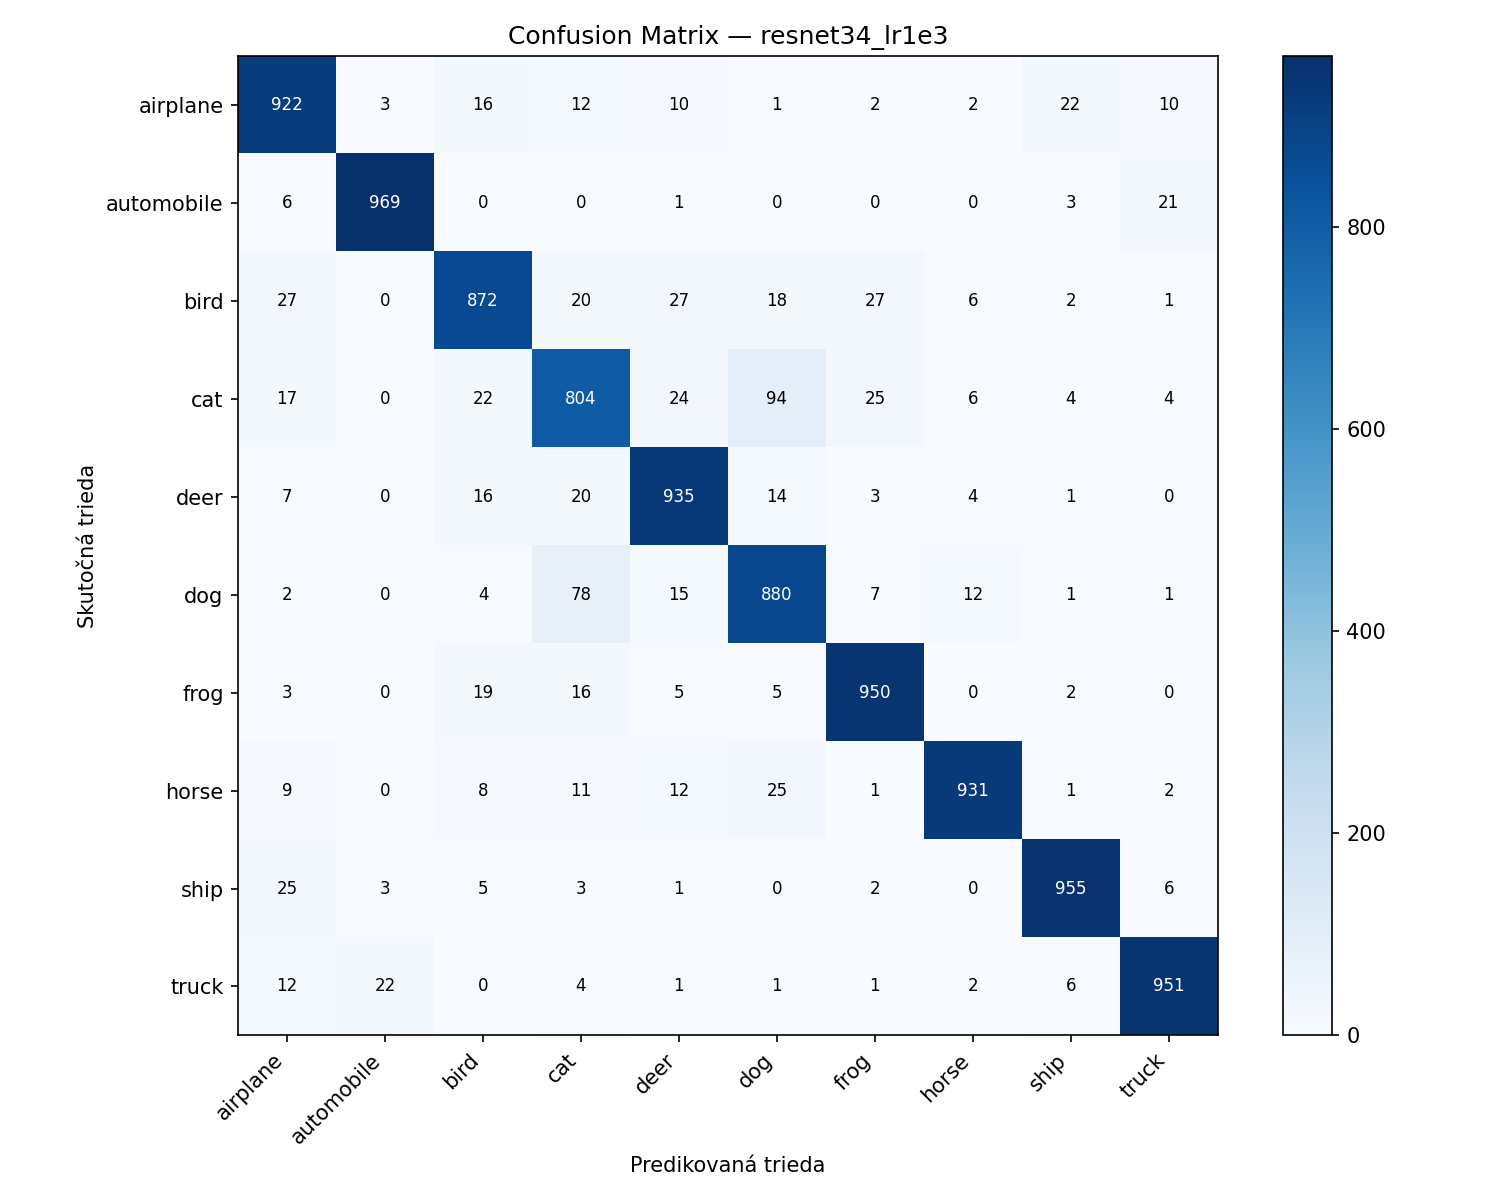
\includegraphics[width=\textwidth]{images/resnet34_lr1e3_confusion_matrix.png}
    \caption{ResNet-34, $lr = 10^{-3}$}
  \end{subfigure}
  \hfill
  \begin{subfigure}[b]{0.48\textwidth}
    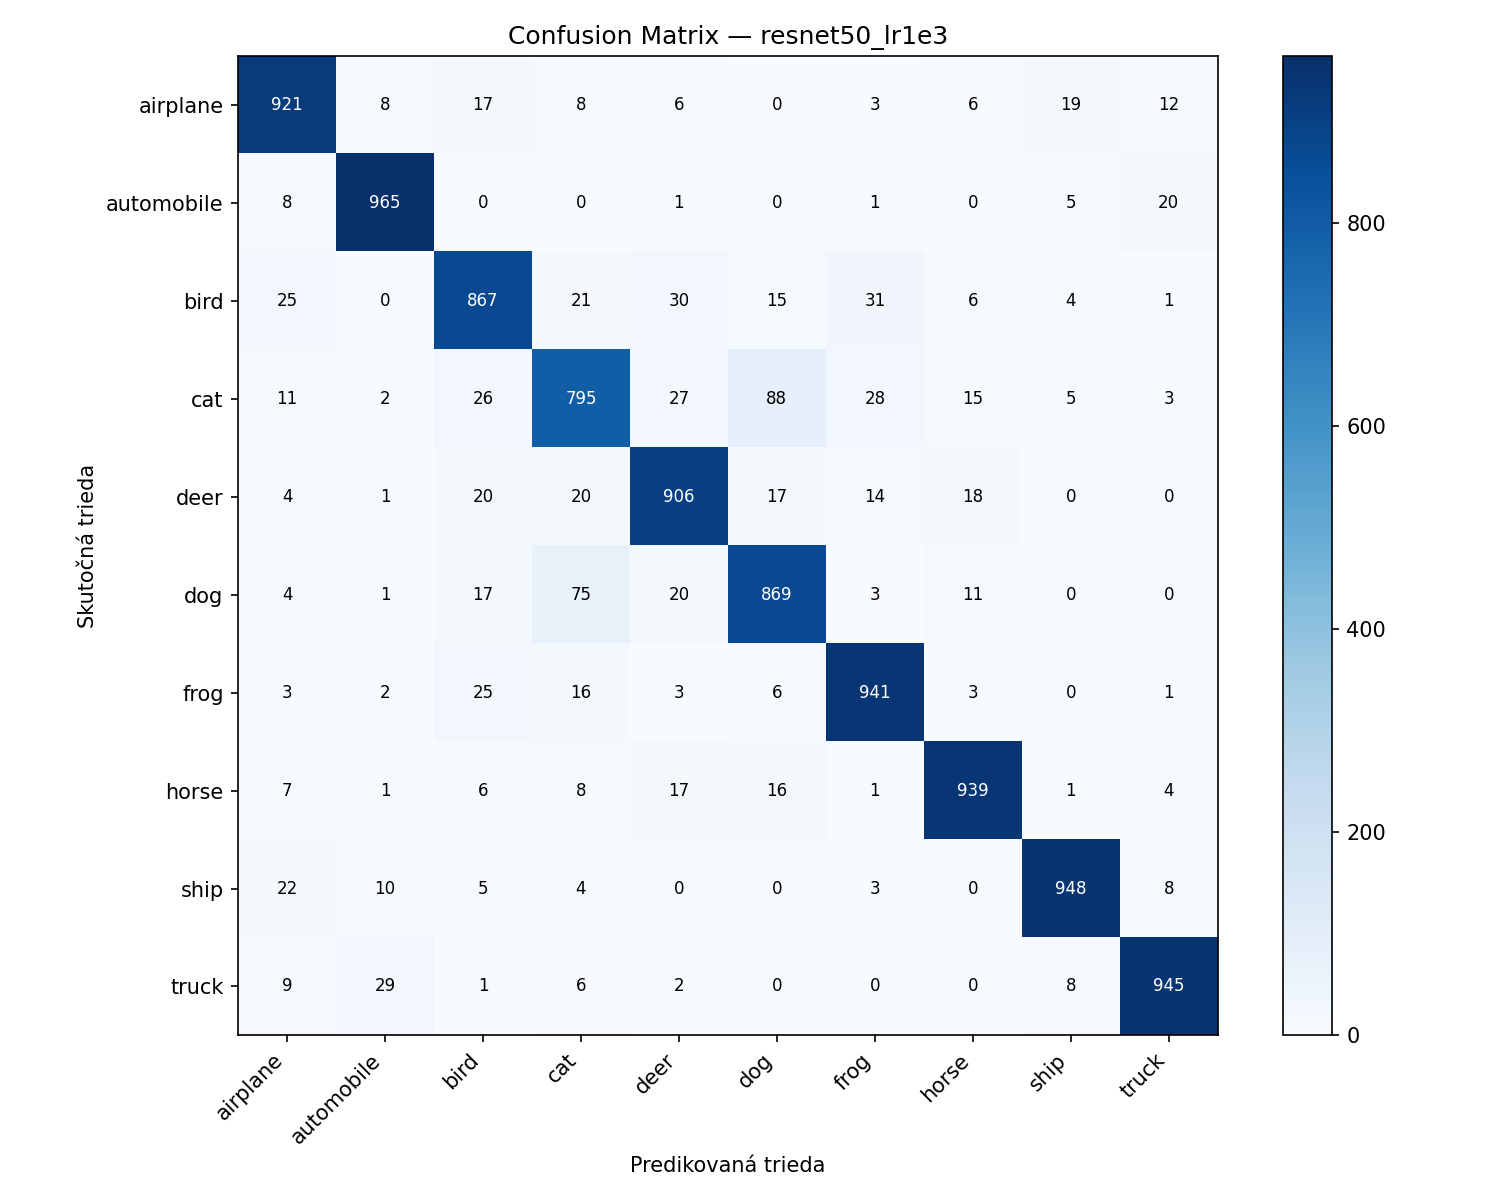
\includegraphics[width=\textwidth]{images/resnet50_lr1e3_confusion_matrix.png}
    \caption{ResNet-50, $lr = 10^{-3}$}
  \end{subfigure}
  \caption{Confusion matrix na testovacej sade (E1 a E3)}
  \label{fig:confusion}
\end{figure}

% ======================================================================
\section{Kritická analýza a diskusia}
% ======================================================================

\subsection{Prečo ResNet-34 predbehol ResNet-50?}

Výsledok môže pôsobiť prekvapivo — menej hlboká sieť dosiahla lepšiu presnosť.
Dôvody sú nasledovné:

\paragraph{1. Overfitting vs. underfitting.}
CIFAR-10 je relatívne jednoduchý dataset (32×32 px, 10 tried). ResNet-50 má
výrazne viac parametrov (bottleneck bloky výrazne zvyšujú kapacitu).
Pri krátkom trénovaní (20 epoch) väčšia kapacita nie je plne využitá
a model sklouzáva do čiastočného overfittingu.

\paragraph{2. Nedostatočný tréning pre väčší model.}
ResNet-50 s $lr = 10^{-3}$ ešte po 20 epochách nebol plne konvergovaný
(train\_acc = 96.98\,\%, zatiaľ čo ResNet-34 dosiahol 97.84\,\%).
Väčší model potrebuje viac epoch alebo vyšší LR, aby plne využil svoju kapacitu.

\paragraph{3. Adaptácia architektúry.}
Obe siete boli adaptované pre CIFAR-10 (zmena conv1 a odstránenie maxpool).
Táto adaptácia sa mierne odlišuje od pôvodného dizajnu bottleneck blokov,
čo môže nepriaznivo ovplyvniť ResNet-50 viac ako ResNet-34.

\subsection{Vplyv rýchlosti učenia (ablačná štúdia)}

Výsledky ablačnej štúdie odhalili zaujímavú asymetriu:

\begin{itemize}
  \item \textbf{ResNet-34}: pokles z $lr = 10^{-3}$ na $10^{-4}$ spôsobil pokles test acc
        o 6.50 p.b. (z 91.69\,\% na 85.19\,\%).
  \item \textbf{ResNet-50}: rovnaký pokles LR spôsobil pokles o 13.71 p.b.
        (z 90.96\,\% na 77.25\,\%).
\end{itemize}

Väčší model je teda \textbf{citlivejší na voľbu rýchlosti učenia}. Vysvetlenie:
pri $lr = 10^{-4}$ s CosineAnnealingLR je počiatočná rýchlosť učenia príliš malá
na to, aby sa hlbší model dostal z oblasti slabej počiatočnej inicializácie.
Gradient norma E4 (32.95 v 1. epoche) potvrdzuje, že sieť sa ocitla v oblasti
ostrého gradientu, avšak LR nestačilo na opustenie tejto oblasti.

\subsection{Pamäť a čas ako praktické kritériá}

Z praktického pohľadu je pomer výkon/zdroje rozhodujúci:
\begin{itemize}
  \item ResNet-50 spotreboval $2.63\times$ viac pamäte za cenu len 0.73 p.b.
        lepšieho výkonu v najlepšom prípade (a dokonca horšieho s rovnakou LR).
  \item Na CIFAR-10 je ResNet-34 \textbf{pareto-optimálnou voľbou}: nižšia pamäť,
        kratší čas trénovania, mierne lepšia presnosť.
  \item Na náročnejšom datasete (ImageNet, CIFAR-100) by porovnanie mohlo byť
        odlišné, keďže väčšia kapacita ResNet-50 by mala väčší priestor sa prejaviť.
\end{itemize}

\subsection{Analýza chýb — ktoré triedy sú najťažšie?}

Zo všetkých experimentov konzistentne vyplýva, že najťažšie triedy sú:
\begin{enumerate}
  \item \textbf{cat} (80.4\,\% a 79.5\,\%) — najčastejšie zamieňaná s dog
  \item \textbf{bird} (87.2\,\% a 86.7\,\%)
  \item \textbf{dog} (88.0\,\% a 86.9\,\%)
\end{enumerate}
Tieto triedy zdieľajú vizuálne rysy: cat a dog majú podobné tvary tela a srsti,
bird môže byť zamieňaný s letúchom (airplane) pri nízkom rozlíšení.
Najľahšie triedy sú \textbf{automobile, ship, truck} — vozidlá majú charakteristické
geometrické tvary, ktoré sú jednoznačné aj na 32×32 px obrázkoch.

\subsection{Stabilita učenia a skip connections}

Gradient norma E1 a E3 klesá monotónne od $\approx 3.5$ (resp. $4.2$) na $\approx 1.2$
(resp. $1.5$), čo svedčí o stabilnom toku gradientu — priamym dôsledkom reziduálnych
prepojení. V experimente E4 vysoká počiatočná gradient norma (32.95) ukazuje, že bez
správnej kalibrácie LR môže aj sieť so skip connections trpieť nestabilitou.

% ======================================================================
\section{Obmedzenia a možnosti ďalšej práce}
% ======================================================================

\paragraph{Obmedzenia tejto štúdie:}
\begin{itemize}
  \item \textbf{Krátke trénovanie (20 epoch):} Oba modely s $lr = 10^{-3}$ ešte
        nedosiahli plnú konvergenciu; dlhší tréning by mohol zmeniť relatívne porovnanie.
  \item \textbf{Iba dve hodnoty LR:} Grid search alebo Bayesian optimalizácia
        by odhalili optimálne LR pre každú architektúru osobitne.
  \item \textbf{Jednoduchý dataset:} CIFAR-10 nemusí plne využiť kapacitu ResNet-50;
        experimenty na CIFAR-100 alebo Tiny ImageNet by boli informatívnejšie.
  \item \textbf{Bez transfer learningu:} Porovnanie „od nuly" je spravodlivé
        pre architekturálnu analýzu, ale pre praktické nasadenie by bol transfer
        learning relevantnejší.
\end{itemize}

\paragraph{Možnosti ďalšej práce:}
\begin{itemize}
  \item Predĺžiť tréning na 100+ epoch s warm-up fázou.
  \item Porovnať s ResNet-101 a ResNet-152 pre širší pohľad na škálovanie.
  \item Pridať label smoothing alebo mixup augmentáciu.
  \item Vizualizovať aktivačné mapy pomocou Grad-CAM pre interpretovateľnosť.
  \item Otestovať na CIFAR-100 pre porovnanie pri väčšom počte tried.
\end{itemize}

% ======================================================================
\section{Prínosy jednotlivých členov tímu}
% ======================================================================

Projekt riešil \textbf{Marko Zeliznak} (samostatný projekt):
\begin{itemize}
  \item Návrh experimentálnej metodológie a konfigurácia hyperparametrov.
  \item Implementácia tréningového pipeline (adaptácia modelov pre CIFAR-10,
        záznam metrík, ukladanie checkpointov).
  \item Trénovanie všetkých 4 experimentov a generovanie výsledkov.
  \item Analýza chýb (confusion matrix, misclassified samples, per-class accuracy).
  \item Vypracovanie tohto reportu.
\end{itemize}

% ======================================================================
\section{Záver}
% ======================================================================

Táto štúdia porovnávala ResNet-34 a ResNet-50 na datasete CIFAR-10 pri dvoch
konfiguráciách rýchlosti učenia. Hlavné zistenia:

\begin{enumerate}
  \item \textbf{ResNet-34 ($lr = 10^{-3}$) dosiahol najlepší test accuracy (91.69\,\%)}
        napriek menšej hĺbke, čo demonštruje, že väčšia kapacita modelu nezaručuje
        lepšie výsledky pri obmedzenom trénovaní na jednoduchom datasete.
  \item \textbf{Pamäťová a výpočtová náročnosť ResNet-50 je výrazne vyššia}
        ($2.63\times$ viac pamäte, $1.60\times$ dlhší čas epochy) bez zodpovedajúceho
        prínosu v presnosti.
  \item \textbf{ResNet-50 je citlivejší na voľbu LR:} pokles z $10^{-3}$ na $10^{-4}$
        spôsobil stratu 13.71 p.b. vs. 6.50 p.b. pri ResNet-34.
  \item \textbf{Skip connections stabilizujú gradient flow:} gradient normy klesajú
        monotónne u E1 a E3, čo potvrdzuje teóriu o benefitoch reziduálnych prepojení.
  \item \textbf{Najťažšie triedy sú cat, dog, bird} — konzistentne naprieč všetkými
        modelmi, čo odráža inherentnú vizuálnu podobnosť týchto tried na 32×32 px.
\end{enumerate}

Záverom možno konštatovať, že pre jednoduchý experiment na CIFAR-10 je
\textbf{ResNet-34 praktickejšou voľbou}: poskytuje porovnateľnú presnosť s výrazne
nižšou pamäťovou a výpočtovou záťažou. Hlbšie architektúry ako ResNet-50
preukážu svoju hodnotu na náročnejších úlohách, kde väčšia kapacita a dlhšie
trénovanie sú oprávnené.

% ======================================================================
\bibliographystyle{plain}
\bibliography{references}
% ======================================================================

\end{document}